\documentclass[aspectratio=43]{beamer}

% Text packages to stop warnings
\usepackage{lmodern}
\usepackage{textcomp}
\usepackage{tikz}
\usepackage{listings}

% Themes
\usetheme{Boadilla}
\setbeamertemplate{footline}[page number]{}
\setbeamertemplate{navigation symbols}{}

% Suppress the navigation bar
\beamertemplatenavigationsymbolsempty

\lstset{basicstyle=\scriptsize\color{white}, backgroundcolor=\color{black}, rulecolor=\color{black}}

\newenvironment{changemargin}[1]{% 
  \begin{list}{}{% 
    \setlength{\topsep}{0pt}% 
    \setlength{\leftmargin}{#1}% 
    \setlength{\rightmargin}{1em}
    \setlength{\listparindent}{\parindent}% 
    \setlength{\itemindent}{\parindent}% 
    \setlength{\parsep}{\parskip}% 
  }% 
  \item[]}{\end{list}} 

\title{Lecture 04---SMP, Processes vs Threads}
\subtitle{ECE 459: Programming for Performance}
\author{Patrick Lam}
\institute{University of Waterloo}
\date{January 12, 2015}

\begin{document}

%%%%%%%%%%%%%%%%%%%%%%%%%%%%%%%%%%%%%%%%%%%%%%%%%%%%%%%%%%%%%%%%%%%%%%%%%%%%%%%%
\begin{frame}[plain]
  \titlepage
\end{frame}
%%%%%%%%%%%%%%%%%%%%%%%%%%%%%%%%%%%%%%%%%%%%%%%%%%%%%%%%%%%%%%%%%%%%%%%%%%%%%%%%

%%%%%%%%%%%%%%%%%%%%%%%%%%%%%%%%%%%%%%%%%%%%%%%%%%%%%%%%%%%%%%%%%%%%%%%%%%%%%%%%
\begin{frame}
  \frametitle{Last Time: Laws, Thread Models}

  \begin{changemargin}{2cm}
    Amdahl's Law: speedup is bounded by serial part.\\[1em]

    Gustafson's Law: with more resources, \\
    \hspace*{2em}can compute more in same time.\\[2em]
    Thread models: kernel (1:1), user (N:1), hybrid (M:N).
  \end{changemargin}
\end{frame}
%%%%%%%%%%%%%%%%%%%%%%%%%%%%%%%%%%%%%%%%%%%%%%%%%%%%%%%%%%%%%%%%%%%%%%%%%%%%%%%%

%%%%%%%%%%%%%%%%%%%%%%%%%%%%%%%%%%%%%%%%%%%%%%%%%%%%%%%%%%%%%%%%%%%%%%%%%%%%%%%%
\begin{frame}
  \frametitle{Admin}
  \begin{changemargin}{2cm}
  Log on to ecgit by Wednesday and upload your ssh key.\\[2em]
  In case you're interested, this course has 155 students enrolled at the moment (a record).\\[1em]
  SE: 47, NE: 1, MECTR: 11, exchange: 2\\
  ELE: 14, COMPE: 80.
  \end{changemargin}

\end{frame}
%%%%%%%%%%%%%%%%%%%%%%%%%%%%%%%%%%%%%%%%%%%%%%%%%%%%%%%%%%%%%%%%%%%%%%%%%%%%%%%%

\part{Types of Multiprocessing}
\begin{frame}
  \partpage
\end{frame}

%%%%%%%%%%%%%%%%%%%%%%%%%%%%%%%%%%%%%%%%%%%%%%%%%%%%%%%%%%%%%%%%%%%%%%%%%%%%%%%%
\begin{frame}[fragile]
  \frametitle{Example System---Physical View}
  
  \begin{center}
  \includegraphics[scale=0.25]{L03/computer-parts}
  \end{center}

  \begin{itemize}
    \item Only one physical CPU
  \end{itemize}
\end{frame}
%%%%%%%%%%%%%%%%%%%%%%%%%%%%%%%%%%%%%%%%%%%%%%%%%%%%%%%%%%%%%%%%%%%%%%%%%%%%%%%%

%%%%%%%%%%%%%%%%%%%%%%%%%%%%%%%%%%%%%%%%%%%%%%%%%%%%%%%%%%%%%%%%%%%%%%%%%%%%%%%%
\begin{frame}[fragile]
  \frametitle{Example System---System View}

  \scriptsize
  \begin{lstlisting}
jon@ece459-1 ~ % egrep 'processor|model name' /proc/cpuinfo 
processor : 0
model name: Intel(R) Core(TM) i7-2600K CPU @ 3.40GHz
processor : 1
model name: Intel(R) Core(TM) i7-2600K CPU @ 3.40GHz
processor : 2
model name: Intel(R) Core(TM) i7-2600K CPU @ 3.40GHz
processor : 3
model name: Intel(R) Core(TM) i7-2600K CPU @ 3.40GHz
processor : 4
model name: Intel(R) Core(TM) i7-2600K CPU @ 3.40GHz
processor : 5
model name: Intel(R) Core(TM) i7-2600K CPU @ 3.40GHz
processor : 6
model name: Intel(R) Core(TM) i7-2600K CPU @ 3.40GHz
processor : 7
model name: Intel(R) Core(TM) i7-2600K CPU @ 3.40GHz
  \end{lstlisting}

  \begin{itemize}
    \item Many processors
  \end{itemize}
\end{frame}
%%%%%%%%%%%%%%%%%%%%%%%%%%%%%%%%%%%%%%%%%%%%%%%%%%%%%%%%%%%%%%%%%%%%%%%%%%%%%%%%

%%%%%%%%%%%%%%%%%%%%%%%%%%%%%%%%%%%%%%%%%%%%%%%%%%%%%%%%%%%%%%%%%%%%%%%%%%%%%%%%
\begin{frame}
  \frametitle{SMP (Symmetric Multiprocessing)}

  \begin{changemargin}{2cm}
    Identical processors or cores, which:
    \begin{itemize}
    \item are interconnected, usually using buses; and
    \item share main memory.
    \end{itemize}
    ~\\[1em]
    $\bullet$ SMP is most common type of multiprocessing system.
  \end{changemargin}
\end{frame}
%%%%%%%%%%%%%%%%%%%%%%%%%%%%%%%%%%%%%%%%%%%%%%%%%%%%%%%%%%%%%%%%%%%%%%%%%%%%%%%%

%%%%%%%%%%%%%%%%%%%%%%%%%%%%%%%%%%%%%%%%%%%%%%%%%%%%%%%%%%%%%%%%%%%%%%%%%%%%%%%%
\begin{frame}
  \frametitle{Example of an SMP System}
\begin{center}
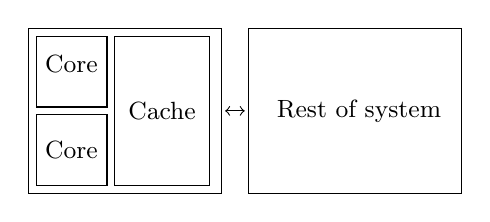
\begin{tikzpicture}
\draw (-0.5, -0.5) rectangle ++(0.9, 0.9);
\draw (-0.05, 0.05) node {\small Core};

\draw (-0.5, -1.5) rectangle ++(0.9, 0.9);
\draw (-0.05, -1.05) node {\small Core};

\draw (0.5, -1.5) rectangle ++(1.2, 1.9);
\draw (1.1, -.55) node {\small Cache};

\draw (-0.6, -1.6) rectangle ++(2.45, 2.1);

\draw (2.2, -1.6) rectangle ++(2.7, 2.1);
\draw (3.6, -0.55) node {\small Rest of system};

\draw[<->] (1.9, -0.55) -- (2.15, -0.55);
\end{tikzpicture}
\end{center}

  \begin{itemize}
    \item Each core can execute a different thread
    \item Shared memory quickly becomes the bottleneck
  \end{itemize}
\end{frame}
%%%%%%%%%%%%%%%%%%%%%%%%%%%%%%%%%%%%%%%%%%%%%%%%%%%%%%%%%%%%%%%%%%%%%%%%%%%%%%%%

%%%%%%%%%%%%%%%%%%%%%%%%%%%%%%%%%%%%%%%%%%%%%%%%%%%%%%%%%%%%%%%%%%%%%%%%%%%%%%%%
\begin{frame}
  \frametitle{Executing 2 Threads on a Single Core}

  \begin{center}
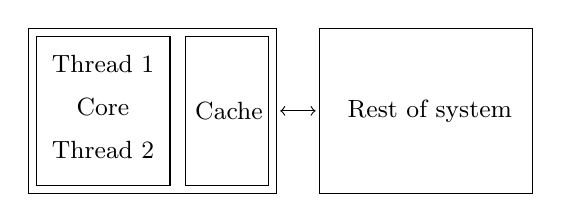
\begin{tikzpicture}
\draw (-1.4, -1.5) rectangle ++(1.7, 1.9);
\draw (-0.55, 0.05) node {\small Thread 1};
\draw (-0.55, -1.05) node {\small Thread 2};
\draw (-0.55, -0.5) node {\small Core};

\draw (0.5, -1.5) rectangle ++(1.05, 1.9);
\draw (1.05, -.55) node {\small Cache};

\draw (-1.5, -1.6) rectangle ++(3.15, 2.1);

\draw (2.2, -1.6) rectangle ++(2.7, 2.1);
\draw (3.6, -0.55) node {\small Rest of system};

\draw[<->] (1.7, -0.55) -- (2.15, -0.55);
\end{tikzpicture}
  \end{center}

  \begin{changemargin}{2.5cm}
    On a single core, must context switch between threads:
      \begin{itemize}
        \item every $N$ cycles; or
        \item wait until cache miss, or another long event
      \end{itemize}
    Resources may be unused during execution. \vfill

    Why not take advantage of this?
  \end{changemargin}
\end{frame}
%%%%%%%%%%%%%%%%%%%%%%%%%%%%%%%%%%%%%%%%%%%%%%%%%%%%%%%%%%%%%%%%%%%%%%%%%%%%%%%%

%%%%%%%%%%%%%%%%%%%%%%%%%%%%%%%%%%%%%%%%%%%%%%%%%%%%%%%%%%%%%%%%%%%%%%%%%%%%%%%%
\begin{frame}
  \frametitle{Executing M Threads on a N Cores}
\begin{center}
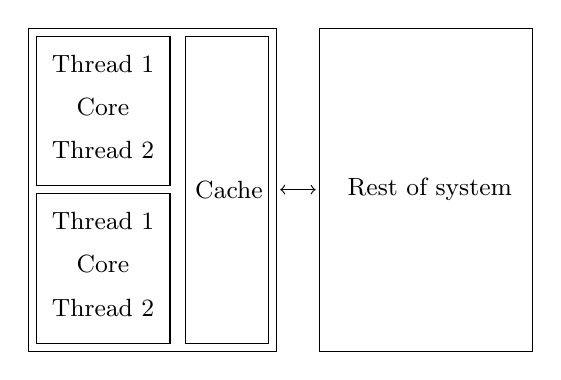
\begin{tikzpicture}

 \draw (-1.4, -1.5) rectangle +(1.7, 1.9);
 \draw (-1.4, -3.5) rectangle +(1.7, 1.9);

\foreach \y in {-2, 0}
{
 \draw (-0.55, 0.05) + (0, \y) node {\small Thread 1};
 \draw (-0.55, -1.05) + (0, \y) node {\small Thread 2};
 \draw (-0.55, -0.5) + (0, \y) node {\small Core};
}

\draw (0.5, -3.5) rectangle ++(1.05, 3.9);
\draw (1.05, -1.55) node {\small Cache};

\draw (-1.5, -3.6) rectangle ++(3.15, 4.1);

\draw (2.2, -3.6) rectangle ++(2.7, 4.1);
\draw (3.6, -1.55) node {\small Rest of system};

\draw[<->] (1.7, -1.55) -- (2.15, -1.55);
\end{tikzpicture}
\end{center}

\begin{changemargin}{2.5cm}
Here's a Chip Multithreading example. \vfill

UltraSPARC T2 has 8 cores, each of which supports 8 
threads. All of the cores share a common level 2 cache.
\end{changemargin}

\end{frame}

%%%%%%%%%%%%%%%%%%%%%%%%%%%%%%%%%%%%%%%%%%%%%%%%%%%%%%%%%%%%%%%%%%%%%%%%%%%%%%%%
\begin{frame}
  \frametitle{SMT (Simultaneous Multithreading)}

  \begin{changemargin}{2.5cm}
    Use idle CPU resources (may be calculating or waiting
          for memory) to execute another task.
    \vfill
    Cannot improve performance if shared resources are the bottleneck.
    \vfill
    Issue instructions for each thread per cycle.
    \vfill
    To the OS, it looks a lot like SMP, but gives only up to 30\% performance improvement.
    \vfill
    \item Intel implementation: Hyper-Threading.
  \end{changemargin}
\end{frame}
%%%%%%%%%%%%%%%%%%%%%%%%%%%%%%%%%%%%%%%%%%%%%%%%%%%%%%%%%%%%%%%%%%%%%%%%%%%%%%%%

%%%%%%%%%%%%%%%%%%%%%%%%%%%%%%%%%%%%%%%%%%%%%%%%%%%%%%%%%%%%%%%%%%%%%%%%%%%%%%%%
\begin{frame}
  \frametitle{Example: Non-SMP system}

\begin{center}
  \includegraphics[height=.5\textheight]{L03/ps3-small}
\end{center}

  PlayStation 3 contains a Cell processor:
  \begin{itemize}
    \item PowerPC main core (Power Processing Element, or ``PPE'')
    \item 7 Synergistic Processing Elements (``SPE''s): small vector computers.
  \end{itemize}
\end{frame}
%%%%%%%%%%%%%%%%%%%%%%%%%%%%%%%%%%%%%%%%%%%%%%%%%%%%%%%%%%%%%%%%%%%%%%%%%%%%%%%%

%%%%%%%%%%%%%%%%%%%%%%%%%%%%%%%%%%%%%%%%%%%%%%%%%%%%%%%%%%%%%%%%%%%%%%%%%%%%%%%%
\begin{frame}
  \frametitle{NUMA (Non-Uniform Memory Access)}

  \begin{changemargin}{2.5cm}
    In SMP, all CPUs have uniform (the same) access time for resources.
    \vfill
    For NUMA, CPUs can access different resources faster (resources: not just
          memory).
    \vfill
    Schedule tasks on CPUs which access resources faster.
    \vfill
    Since memory is commonly the bottleneck, each CPU has its own memory
          bank.
  \end{changemargin}
\end{frame}
%%%%%%%%%%%%%%%%%%%%%%%%%%%%%%%%%%%%%%%%%%%%%%%%%%%%%%%%%%%%%%%%%%%%%%%%%%%%%%%%

%%%%%%%%%%%%%%%%%%%%%%%%%%%%%%%%%%%%%%%%%%%%%%%%%%%%%%%%%%%%%%%%%%%%%%%%%%%%%%%%
\begin{frame}
  \frametitle{Processor Affinity}

  \begin{changemargin}{2cm}
    Each task (process/thread) can be associated with a set of processors.
    \vfill
    Useful to take advantage of existing caches (either from the last time
          the task ran or task uses the same data).
    \vfill
    Hyper-Threading is an example of complete affinity for both threads on
          the same core.
    \vfill
    Often better to use a different processor if current set busy.
  \end{changemargin}
\end{frame}
%%%%%%%%%%%%%%%%%%%%%%%%%%%%%%%%%%%%%%%%%%%%%%%%%%%%%%%%%%%%%%%%%%%%%%%%%%%%%%%%

\part{Processes vs Threads}

%%%%%%%%%%%%%%%%%%%%%%%%%%%%%%%%%%%%%%%%%%%%%%%%%%%%%%%%%%%%%%%%%%%%%%%%%%%%%%%%
\begin{frame}[fragile]
  \partpage
\end{frame}

%%%%%%%%%%%%%%%%%%%%%%%%%%%%%%%%%%%%%%%%%%%%%%%%%%%%%%%%%%%%%%%%%%%%%%%%%%%%%%%%
\begin{frame}[fragile]
  \frametitle{Background}

  \begin{changemargin}{2.5cm}
  Recall the difference between \structure{processes} and 
          \structure{threads}:
  \begin{itemize}
    \item Threads are basically light-weight processes which piggy-back on
          processes' address space.
  \end{itemize} ~\\
  Traditionally (pre-Linux 2.6) you had to use {\tt fork}~(for~processes) and {\tt clone} (for threads).
  \end{changemargin}

\end{frame}
%%%%%%%%%%%%%%%%%%%%%%%%%%%%%%%%%%%%%%%%%%%%%%%%%%%%%%%%%%%%%%%%%%%%%%%%%%%%%%%%

%%%%%%%%%%%%%%%%%%%%%%%%%%%%%%%%%%%%%%%%%%%%%%%%%%%%%%%%%%%%%%%%%%%%%%%%%%%%%%%%
\begin{frame}[fragile]
  \frametitle{History}

  \begin{changemargin}{2.5cm}
    {\tt clone} is not POSIX compliant.
    ~\\
    Developers mostly used {\tt fork} in the past, which creates a new process.
      \begin{itemize}
        \item Drawbacks?
        \item Benefits?
      \end{itemize}
  \end{changemargin}
\end{frame}
%%%%%%%%%%%%%%%%%%%%%%%%%%%%%%%%%%%%%%%%%%%%%%%%%%%%%%%%%%%%%%%%%%%%%%%%%%%%%%%%

%%%%%%%%%%%%%%%%%%%%%%%%%%%%%%%%%%%%%%%%%%%%%%%%%%%%%%%%%%%%%%%%%%%%%%%%%%%%%%%%
\begin{frame}[fragile]
  \frametitle{Benefit: {\tt fork} is Safer and More Secure Than Threads}

  \begin{changemargin}{1cm}
  \begin{enumerate}
    \item Each process has its own virtual address space:
      \begin{itemize}
        \item Memory pages are not copied, they are copy-on-write---
        \item Therefore, uses less memory than you would expect.
      \end{itemize}
    \item Buffer overruns or other security holes do not expose other~processes.
    \item If a process crashes, the others can continue.
  \end{enumerate}~\\[1em]
  {\bf Example:} In the Chrome browser, each tab is a separate process.
  \end{changemargin}
\end{frame}
%%%%%%%%%%%%%%%%%%%%%%%%%%%%%%%%%%%%%%%%%%%%%%%%%%%%%%%%%%%%%%%%%%%%%%%%%%%%%%%%

%%%%%%%%%%%%%%%%%%%%%%%%%%%%%%%%%%%%%%%%%%%%%%%%%%%%%%%%%%%%%%%%%%%%%%%%%%%%%%%%
\begin{frame}[fragile]
  \frametitle{Drawback of Processes: Threads are Easier and Faster}

  \begin{changemargin}{1cm}
  \begin{itemize}
    \item Interprocess communication (IPC) is more complicated and slower than interthread
          communication.
      \begin{itemize}
        \item Need to use operating system utilities (pipes, semaphores, shared
              memory, etc) instead of thread library (or just memory reads and writes).
      \end{itemize}
    \item Processes have much higher startup, shutdown and synchronization cost.
    \item And, \structure{Pthreads}/\structure{C++11 threads} fix issues\\ with {\tt clone} and provide a
          uniform interface for most systems {\bf (Assignment 1)}.
  \end{itemize}
  \end{changemargin}

\end{frame}
%%%%%%%%%%%%%%%%%%%%%%%%%%%%%%%%%%%%%%%%%%%%%%%%%%%%%%%%%%%%%%%%%%%%%%%%%%%%%%%%

%%%%%%%%%%%%%%%%%%%%%%%%%%%%%%%%%%%%%%%%%%%%%%%%%%%%%%%%%%%%%%%%%%%%%%%%%%%%%%%%
\begin{frame}[fragile]
  \frametitle{Appropriate Time to Use Processes}

  \begin{changemargin}{1cm}
  If your application is like this:
  \begin{itemize}
    \item Mostly independent tasks, with little or no communication.
    \item Task startup and shutdown costs are negligible compared to overall runtime.
    \item Want to be safer against bugs and security holes.
  \end{itemize}
  Then processes are the way to go. \\[1em]

  For performance reasons, along with ease and consistency, we'll use
  \structure{Pthreads}.
  \end{changemargin}

\end{frame}
%%%%%%%%%%%%%%%%%%%%%%%%%%%%%%%%%%%%%%%%%%%%%%%%%%%%%%%%%%%%%%%%%%%%%%%%%%%%%%%%

%%%%%%%%%%%%%%%%%%%%%%%%%%%%%%%%%%%%%%%%%%%%%%%%%%%%%%%%%%%%%%%%%%%%%%%%%%%%%%%%
\begin{frame}[fragile]
  \frametitle{Live coding: overheads of threads vs fork}
\end{frame}
%%%%%%%%%%%%%%%%%%%%%%%%%%%%%%%%%%%%%%%%%%%%%%%%%%%%%%%%%%%%%%%%%%%%%%%%%%%%%%%%

  %%%%%%%%%%%%%%%%%%%%%%%%%%%%%%%%%%%%%%%%%%%%%%%%%%%%%%%%%%%%%%%%%%%%%%%%%%%%%%%%
\begin{frame}[fragile]
  \frametitle{Results: Threads Offer a Speedup of 6.5 over {\tt fork}}

  \begin{changemargin}{1cm}
  Here's a benchmark between {\tt fork} and Pthreads on a laptop, creating and
  destroying 50,000 threads:
  \vfill
  \begin{lstlisting}[basicstyle=\scriptsize]
jon@riker examples master % time ./create_fork 
0.18s user 4.14s system 34% cpu 12.484 total
jon@riker examples master % time ./create_pthread 
0.73s user 1.29s system 107% cpu 1.887 total
  \end{lstlisting}
  \vfill
  Clearly Pthreads incur much lower overhead than {\tt fork}.
  \end{changemargin}
\end{frame}
%%%%%%%%%%%%%%%%%%%%%%%%%%%%%%%%%%%%%%%%%%%%%%%%%%%%%%%%%%%%%%%%%%%%%%%%%%%%%%%%

\end{document}
